\documentclass[english,onecolumn]{IEEEtran}

\usepackage[T1]{fontenc}
\usepackage[latin9]{luainputenc}
\usepackage[letterpaper]{geometry}
\geometry{verbose}
\usepackage{babel}
\usepackage{extarrows}
\usepackage[colorlinks]{hyperref}
\usepackage{listings}
\usepackage{color,xcolor}
\usepackage{graphicx}
\usepackage{subfigure} 
\usepackage{amsthm,amssymb,amsfonts}
\usepackage{textcomp}
\usepackage{bm}
\usepackage{booktabs}

\providecommand{\U}[1]{\protect\rule{.1in}{.1in}}
\topmargin            -18.0mm
\textheight           226.0mm
\oddsidemargin      -4.0mm
\textwidth            166.0mm
\def\baselinestretch{1.5}

\DeclareMathAlphabet\mathbfcal{OMS}{cmsy}{b}{n}
\newcommand{\Ab}{\mathbf{A}}
\newcommand{\Bb}{\mathbf{B}}
\newcommand{\Ub}{\mathbf{U}}
\newcommand{\Vb}{\mathbf{V}}
\newcommand{\ub}{\mathbf{u}}
\newcommand{\vb}{\mathbf{v}}
\newcommand{\Ucal}{\mathbfcal{U}}
\newcommand{\Wcal}{\mathbfcal{W}}
\newcommand{\Vcal}{\mathbfcal{V}}
\newcommand{\Xcal}{\mathbfcal{X}}
\newcommand{\Ycal}{\mathbfcal{Y}}
\newcommand{\Rbb}{\mathbb{R}}

\begin{document}

\begin{center}
	\textbf{\LARGE{SI114H-Computational Science and Engineering, 2025 Spring}}\\
	{\Large Homework Set \#3}\\
\par\end{center}

\noindent
\rule{\linewidth}{0.4pt}
{\bf Requirements:}
\begin{enumerate}
	\item Deadline: {\bf \textcolor{red}{11pm, 17 May 2025}}. %Homework\#2 only contains the programming part.

	\item About your codes:
	\begin{enumerate}
	    \item Make sure that your codes can run and are consistent with your results.
	    \item Attach a {\textcolor{blue}{Readme.txt}} file to clearly identify the function of each file.
	\end{enumerate}

 \item You need to compress three files \textbf{code} , \textbf{readme} (Add supplementary explanations to the code), and \textbf{PDF} (Show your results) into one file, name this file as \textcolor{blue}{student ID + your name} and send it to the blackboard system.

\end{enumerate}
\rule{\linewidth}{0.4pt}



\noindent\textbf{Problem 1}. \textcolor{red}{(50 points)} \par
Find the Fourier series on $-\pi \leq x \leq \pi$ for
\begin{itemize}
	\item[(a)] $f(x) = \sin^3x$, an odd function
	\item[(b)] $f(x) = |\sin x |$, an even function
	\item[(c)] $f(x) = x$
	\item[(d)] $f( x) = e^x$ , using the complex form of the series.
\end{itemize}


\subsection{Solution}

\begin{itemize}
	\item[(a)] $f(x) = \sin^3x$, an odd function\\
	Since $f(x)$ is odd, all cosine coefficients $a_n = 0$. For the sine coefficients:\\

	$\sin^3 x = \sin x \cdot \sin^2 x = \sin x \cdot \frac{1-\cos 2x}{2} = \frac{\sin x - \sin x\cos 2x}{2}$

	Using the identity $\sin A \cos B = \frac{1}{2}[\sin(A+B) + \sin(A-B)]$: $\sin x\cos 2x = \frac{1}{2}[\sin(x+2x) + \sin(x-2x)] = \frac{1}{2}[\sin 3x - \sin x]$

	Therefore: $\sin^3 x = \frac{\sin x - \frac{1}{2}[\sin 3x - \sin x]}{2} = \frac{3\sin x - \sin 3x}{4}$

	So the Fourier series is: $f(x) = \frac{3}{4}\sin x - \frac{1}{4}\sin 3x$

	\item[(b)] $f(x) = |\sin x|$, an even function \\
	Since $f(x)$ is even, all sine coefficients $b_n = 0$. For the constant term and cosine coefficients:\\

	$a_0 = \frac{1}{\pi}\int_{-\pi}^{\pi}|\sin x|dx = \frac{2}{\pi}\int_{0}^{\pi}|\sin x|dx = \frac{2}{\pi}\int_{0}^{\pi}\sin x dx = \frac{2}{\pi}[2] = \frac{4}{\pi}$

	$a_n = \frac{1}{\pi}\int_{-\pi}^{\pi}|\sin x|\cos(nx)dx$

	For odd $n$, these integrals are zero due to symmetry. For even $n$ ($n = 2k$), $a_{2k} = \frac{-4}{\pi}\frac{1}{4k^2-1}$

	The Fourier series is: $f(x) = \frac{2}{\pi} - \frac{4}{\pi}\sum_{k=1}^{\infty}\frac{\cos(2kx)}{4k^2-1}$

	\item[(c)] $f(x) = x$\\
	This is neither even nor odd, so we need both sine and cosine terms:\\

	$a_0 = \frac{1}{2\pi}\int_{-\pi}^{\pi}x dx = 0$

	$a_n = \frac{1}{\pi}\int_{-\pi}^{\pi}x\cos(nx)dx = 0$ for all $n$ (can be shown by integration by parts)

	$b_n = \frac{1}{\pi}\int_{-\pi}^{\pi}x\sin(nx)dx = \frac{2(-1)^{n+1}}{n}$

	The Fourier series is: $f(x) = 2\sum_{n=1}^{\infty}\frac{(-1)^{n+1}}{n}\sin(nx) = 2[\sin x - \frac{\sin 2x}{2} + \frac{\sin 3x}{3} - ...]$

	\item[(d)] $f(x) = e^x$ using the complex form\\
	For the complex Fourier series $f(x) = \sum_{n=-\infty}^{\infty}c_n e^{inx}$:\\

	$c_n = \frac{1}{2\pi}\int_{-\pi}^{\pi}e^x e^{-inx}dx = \frac{1}{2\pi}\int_{-\pi}^{\pi}e^{x-inx}dx$

	$c_n = \frac{1}{2\pi}\left[\frac{e^{x-inx}}{1-in}\right]_{-\pi}^{\pi} = \frac{1}{2\pi}\frac{e^{\pi-in\pi}-e^{-\pi+in\pi}}{1-in} = \frac{e^{\pi}(-1)^n-e^{-\pi}(-1)^n}{2\pi(1-in)}$

	$c_n = \frac{(-1)^n(e^{\pi}-e^{-\pi})}{2\pi(1-in)} = \frac{(-1)^n \cdot 2\sinh(\pi)}{2\pi(1-in)} = \frac{(-1)^n\sinh(\pi)}{\pi(1-in)}$

	Therefore, the complex Fourier series is: $f(x) = \sum_{n=-\infty}^{\infty}\frac{(-1)^n\sinh(\pi)}{\pi(1-in)}e^{inx}$

\end{itemize}

\noindent\textbf{Problem 2}. \textcolor{red}{(50 points)} \par
Show the Gibbs phenomenon using a numerical example. 


Gibbs Phenomenon Demonstration:\\
The plot shows the Fourier series approximation of a square wave.\\
Notice the overshoot and undershoot near the discontinuities (t=0, t=pi, t=-pi).\\
As the number of terms (N) increases, the approximation gets better overall,
but the height of the overshoot remains significant (approx. 9\% of the jump),
though it gets squeezed into a narrower region around the discontinuity.

\begin{figure}[h]
	\centering
	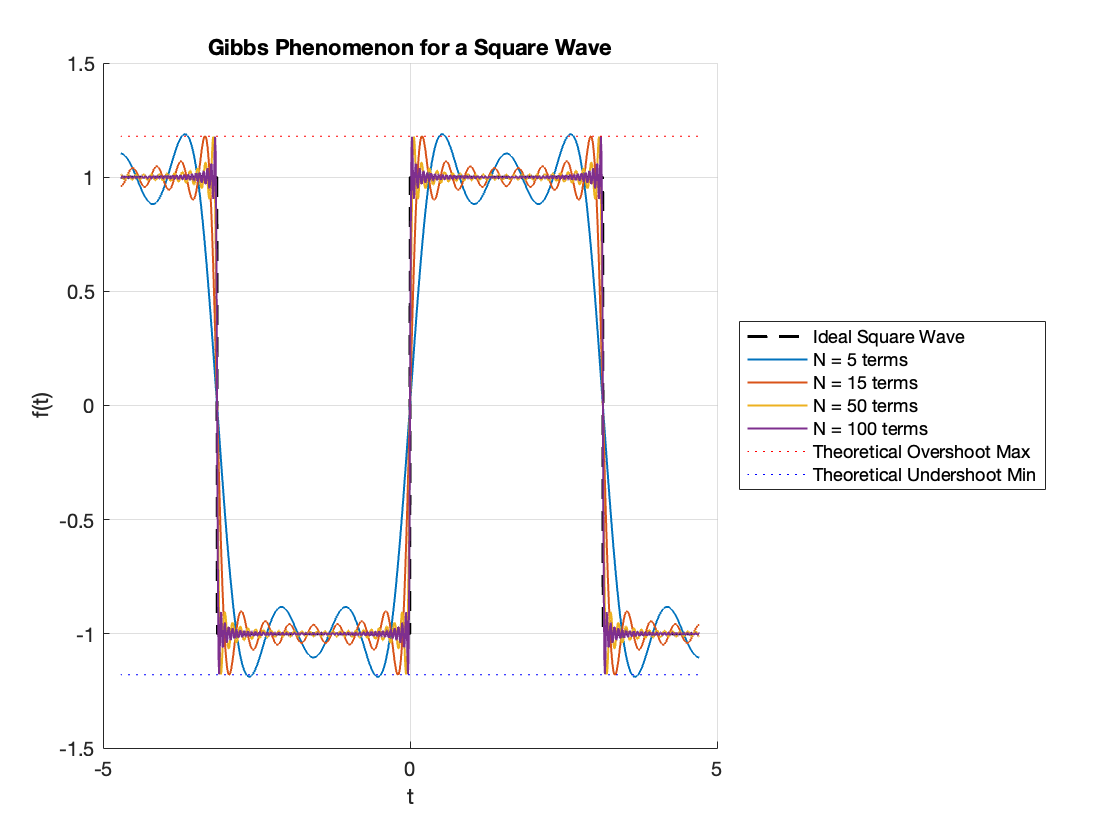
\includegraphics[width=0.6\textwidth]{Gibbs.png}
	\caption{Gibbs Phenomenon}
	\label{fig:gibbs}
\end{figure}
\end{document}
